\section{Results}
\label{sec:results}

\subsection{Final Model}

The effects in the model are as follows: Intercept, BUILTYR, METRO, NUMBED, LNPROPTX, LNPROPTX*METRO, STATELBL METRO*STATELBL, and LNPROPTX*STATELBL.

\begin{table}[ht]
\scriptsize
\centering
\caption{Final Model Statistics}
\begin{tabular}{|c|c|l}
\hline
Root MSE       & 0.59124     \\
\hline
Dependent Mean & 12.71301    \\
\hline
R-Square       & 0.4960      \\
\hline
Adj R-Sq       & 0.4944      \\
\hline
AIC            & -3836.11727 \\
\hline
AICC           & -3834.59265 \\
\hline
BIC            & -83795      \\
\hline
C(p)           & 1164.65786  \\
\hline
PRESS          & 28100       \\
\hline
SBC            & -81517      \\
\hline
ASE (Train)    & 0.34849     \\
\hline
ASE (Test      & 0.35099     \\
\hline
\end{tabular}
\end{table}


\subsection{Analysis}

The final model that was chosen best predicts home value was found using the step wise selection procedure with p-value as the selection criteria. The predictor variables of age of structure, metropolitan status, number of bedrooms, log value of property tax, log value of property tax interacting with metropolitan status, state, metropolitan status interacting with state, and log value of property tax interacting with state all have significant effect on the dependent house value variable. As referenced in Table I, this model had a test MSE value of 0.59124 which was similar to the other selection criteria we tested. However, this model had the least amount of variables with 8 significant predictors compared to step-wise BIC which had 11 variables and step-wise CP which had 12 variables. The simpler model can more easily analyze single variables and their affects on home value.The forward and backward selection processes using the criteria of p-value both had 8 predictor variables but was slightly less effective in predicting home value. 

\indent The goodness of fit of the model is 0.4944 which is represented by the adjusted R-squared value. This model will accurately predict home value 49.44\% of the time. The model has an f-value of 335.00 with a p-value of less than 0.0001 making at least one of the variables significant in predicting home value.

Fig. \ref{figure:residual_plot} shows an overview of the house count in each state from the simple random sample (SRS) of 100,000 data entries.
Fig. \ref{figure:qq_plot} shows an overview of the house count in each state from the simple random sample (SRS) of 100,000 data entries.

\subsection{Assumptions}
While the final model found significant variables that were accurate predictors of house value, it is important to note that this model does not satisfy the necessary assumptions in order to be accurately used for this prediction. The Normal Q-Q plot shown in Fig. \ref{figure:qq_plot} suggests that the LNValue variable is left skewed and does not follow the normal distribution of data. The residual line varies greatly from the predicted LNValue line. The residual plot presents a heteroscedastic (funneling shape) pattern which violates both the linearity and equal variance assumptions. This in combination with a presence of outliers towards the negative residual values prevents this model from accurately representing the data and its usage as a predictive method.

\begin{figure}[h!]
	\centering
	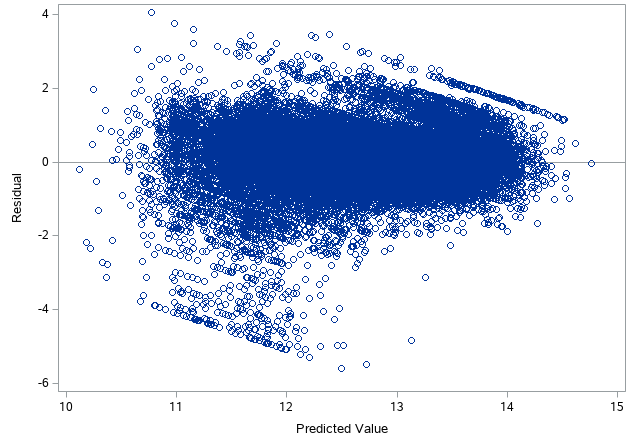
\includegraphics[width=3.5in]{./fig/ResidualPlot.PNG}
	\caption{Residual vs. Predicted Plot of LNVALUE}
	\label{figure:residual_plot}
\end{figure}

\begin{figure}[h!]
	\centering
	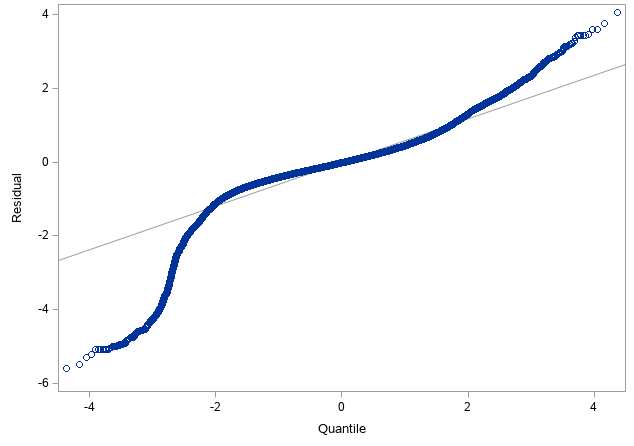
\includegraphics[width=3.5in]{./fig/QQPlot.PNG}
	\caption{Normal Q-Q Plot of LNVALUE}
	\label{figure:qq_plot}
\end{figure}
